\chapter{System Architecture and Design}\label{chap:system_architecture_rewrite}

Chapter~\ref{chap:background} introduced the methods and platform constraints that shape the thesis.
This chapter explains the design decisions behind the proposed scene-aware dialogue system: why it is distributed, how visual observations become persistent scene memory, and how that memory grounds dialogue.
Chapter~\ref{chap:server_side_rewrite} then describes the server implementation, while Chapter~\ref{chap:robot_side_rewrite} describes the Pepper client.
The code is publicly available at \url{https://github.com/JakubCiesko/pepper-ot}.

\section{Design Goals and Constraints}\label{sec:architecture-goals}

The system was designed around the constraints of using Pepper as an embodied dialogue platform.
As discussed in Section~\ref{sec:pepper-specification}, Pepper is suitable as the social and physical interface, but the visual and language inference stack must run externally.

The first design goal is grounding: spoken claims should be backed by detected objects, explicit attributes, and relations stored in the current scene state.
The second goal is persistence: the robot needs memory that survives beyond one camera frame so that later turns can refer to earlier observations.
The third goal is interaction robustness: perception and model calls may be slow or fail, so the client must stay responsive while the server remains inspectable and configurable for experimentation.

\section{Distributed Client--Server Architecture}\label{sec:architecture-client-server}

\begin{figure}[t]
\centering
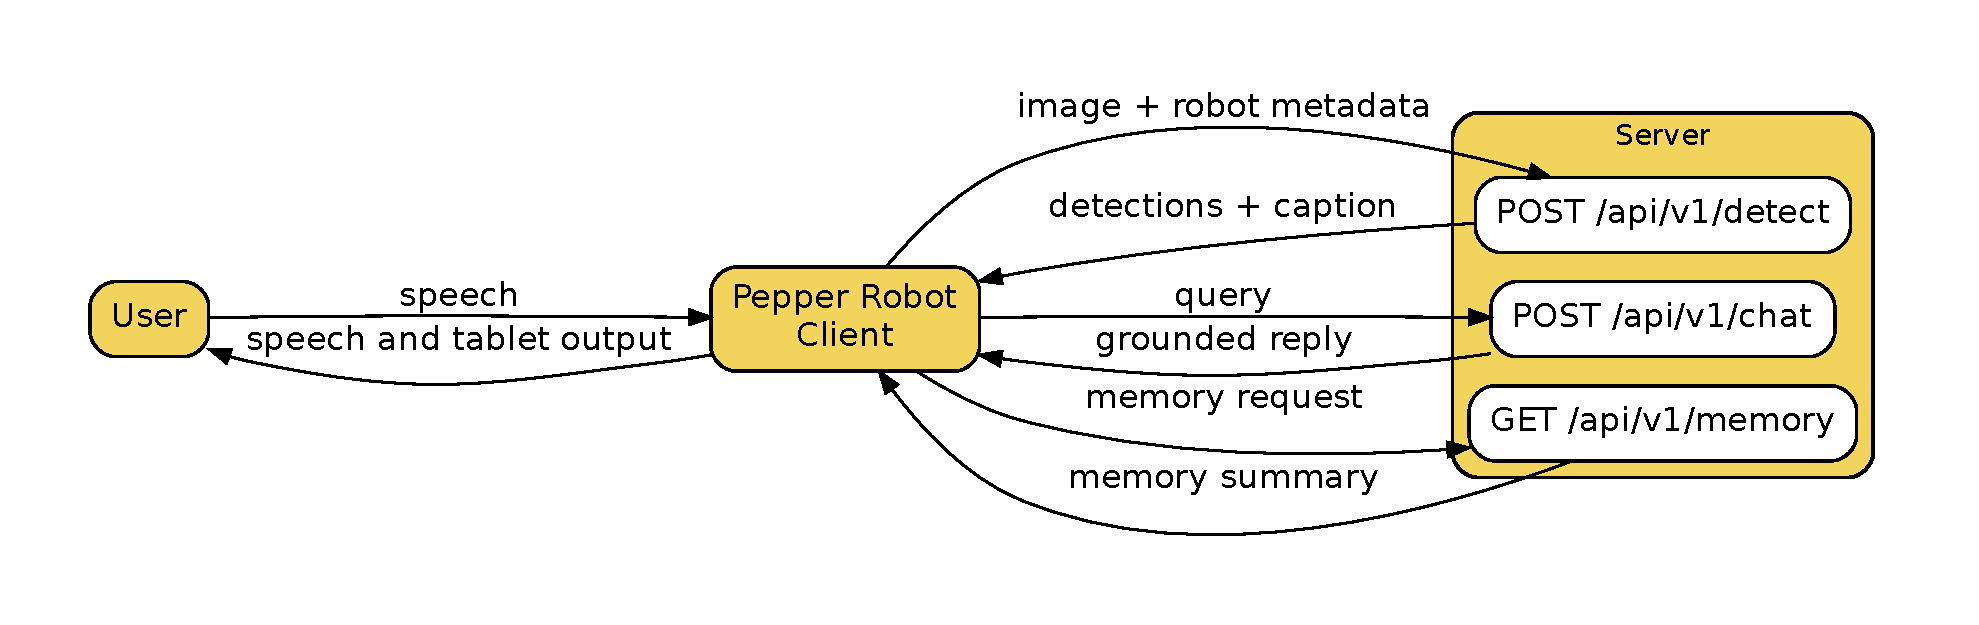
\includegraphics[width=1\linewidth]{pics/architecture.pdf}
\caption{High-level architecture of the proposed scene-aware dialogue system. The Pepper robot client handles user speech input, speech and tablet output, image capture, and robot metadata collection. The server exposes perception, chat, and memory services that create and use the scene representation.}
\label{fig:overall-system-architecture}
\end{figure}

The system follows the distributed architecture shown in Figure~\ref{fig:overall-system-architecture}.
Pepper acts as the embodied client.
It listens to the user through QiChat, captures images, collects robot metadata, sends requests to the server, speaks answers, and updates the tablet.
The server owns the computationally expensive and persistent parts of the system: perception, scene graph generation, scene memory, language-model calls, configuration, and monitoring.

This split is intentionally strict.
The Pepper client does not need to know which detector, VLM, LLM, or scene graph backend is active.
It depends only on stable request and response contracts.
Model experimentation stays on the server side, where GPU resources, worker processes, logs, and dashboard controls are available.

The boundary between the two sides is also designed around the physical robot.
Visual requests carry images with robot metadata; dialogue requests carry the user query and optional object focus.
The server returns captions, memory summaries, grounded answers, or updated scene state, which Pepper presents through speech and the tablet.

\section{Interaction Modes and Data Flow}\label{sec:architecture-data-flow}

The architecture supports several interaction modes because not every user request requires the same amount of perception.
A quick look is the low-latency path: Pepper captures one image and asks for a caption, while heavier memory updates may continue in the background.
A full scan is the memory-building path: the robot observes the room from multiple head poses, and the server updates persistent objects, attributes, and relations.

General questions use the current scene memory without necessarily taking a new image.
Object-focused questions add a recognized object label, allowing the server to build a narrower context around matching objects and neighboring relations.
Finally, memory display exposes the robot's current belief state: Pepper mirrors the interaction-relevant subset into QiChat dynamic concepts and can show a compact summary on the tablet.

\section{Perception and Scene-Graph Pipeline Design}\label{sec:architecture-perception-pipeline}

\begin{figure}[p]
\centering
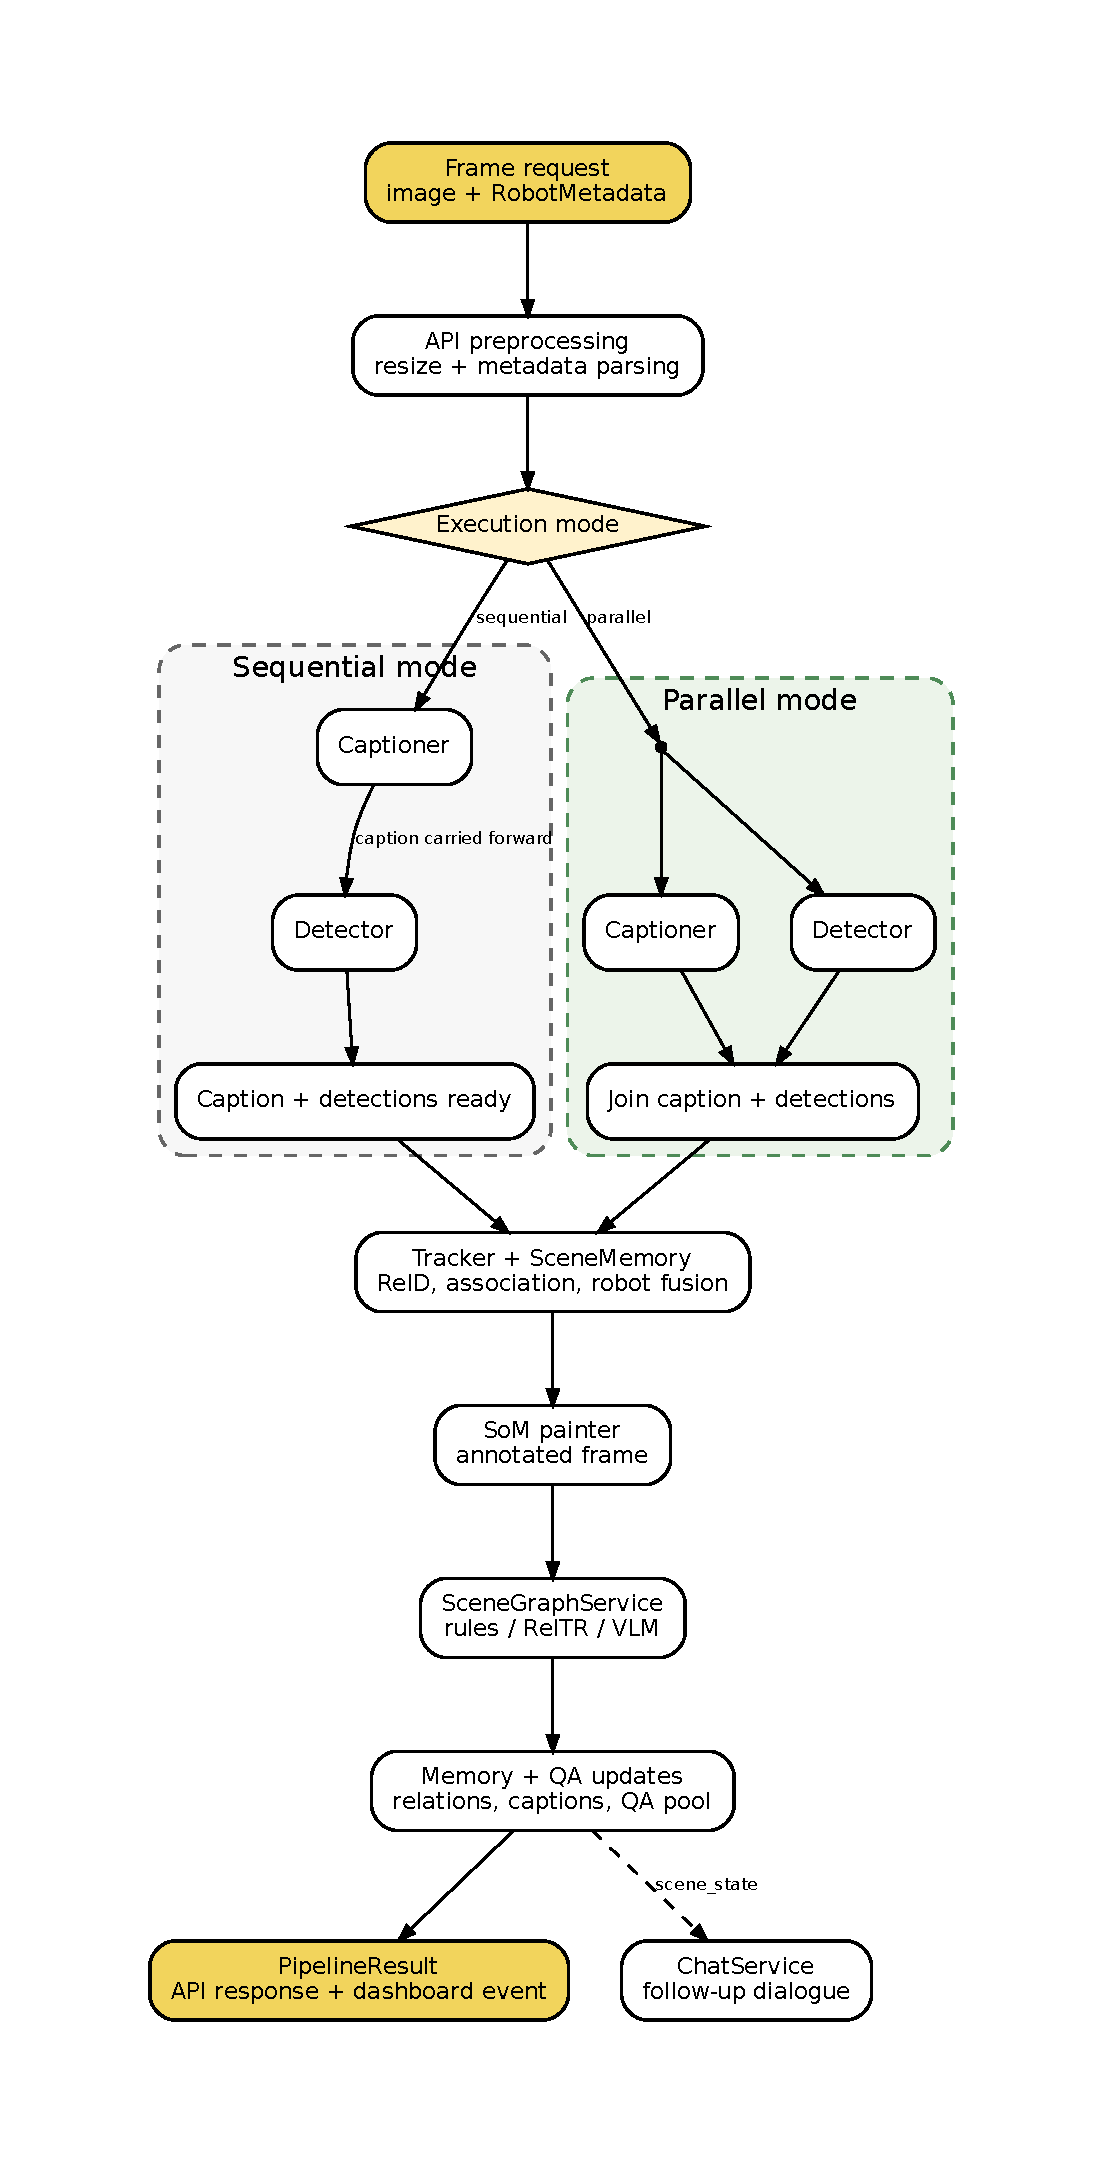
\includegraphics[height=0.86\textheight]{pics/pipeline_less_detailed.pdf}
\caption{High-level perception and memory pipeline. A robot observation can produce a fast caption, detected objects, persistent identities, Set-of-Mark images, scene graph relations, pregenerated questions, and memory updates.}
\label{fig:architecture-perception-pipeline}
\end{figure}

Figure~\ref{fig:architecture-perception-pipeline} shows the perception pipeline at the design level.
The input is a robot observation: an image together with metadata about the camera, head pose, capture mode, and available robot perception signals.
One branch produces a fast caption for immediate speech; another detects objects and creates the grounding layer used by memory and dialogue.

After detection, object association connects frame-local detections to persistent memory entries.
Scene graph generation is then built over these grounded objects.
The system can combine geometric rules, RelTR, VLM-based relation generation, and robot-native metadata about people.
The robot metadata path is important for social relations and attributes that may not be visible from pixels alone, such as distance from Pepper, engagement, waving, or looking at the robot.
No relation source is treated as final authority; generated relations are normalized, filtered, merged, and stored in scene memory.

Set-of-Mark prompting is the grounding mechanism for the VLM path described in Section~\ref{sec:set-of-mark}.
The server can render persistent object identifiers, labels, boxes, masks, or polygons into the image so that the prompt asks for relations between known object instances rather than an unconstrained caption.
The pipeline outputs updated memory, captions, object records, relations, attributes, and optionally pregenerated questions, all of which can be reused by later dialogue turns, the tablet, and the evaluation in Chapter~\ref{chap:experiment}.

\section{Scene Memory as the Central Abstraction}\label{sec:architecture-scene-memory}

Scene memory is the main abstraction between perception and dialogue.
Raw detections are tied to one image, while dialogue needs stable references over time.
The memory therefore stores grounded objects, relations, captions, robot-derived person facts, and cached question-answer pairs.
It is the authoritative representation of what the robot currently knows about the scene.

This design avoids two competing world models.
The server maintains the complete scene state, because it is the component that runs perception, relation generation, and language-model context construction.
The robot client mirrors only the interaction-relevant subset, such as object labels, relation names, attributes, and cached questions.
Those mirrored values are used to update QiChat dynamic concepts and the tablet display, but the full structured memory remains on the server.

The memory representation also gives the language model a controlled source of grounding.
Instead of passing the whole image history into every dialogue turn, the server serializes selected objects, attributes, relations, and recent captions into a compact context.
This context can be further restricted for object-focused questions.
The language model is therefore asked to answer from the scene state rather than from an unconstrained description of the image or from its parametric knowledge alone.

The same abstraction supports inspection and correction.
Because objects and relations are stored explicitly, the dashboard can show the current memory, the robot can display a memory summary, and the experiments can evaluate generated scene graphs against human annotations.
For this reason, scene memory is treated as a first-class component of the architecture rather than as a temporary by-product of detection.

\section{Robot Dialogue Layer}\label{sec:architecture-dialogue-layer}

The robot-side dialogue layer is deliberately not an open-ended LLM loop.
QiChat remains the deterministic front-end that decides which system action should be called.
It recognizes whether the user wants the robot to look, scan, answer a general question, answer a question about a remembered object, display memory, reset memory, or speak a cached answer.
Only after this intent is known does the system call the server and, when needed, a language model.

This design keeps the embodied interaction controllable.
The robot must coordinate speech, head motion, image capture, tablet updates, and network requests.
If every utterance were sent directly to a language model, the model would also need to decide when the robot should move, when it should capture an image, and which local API should be called.
In this system, QiChat and the robot client keep control of actions, while the server language model is used for grounded response generation.

Dynamic concepts connect the changing scene memory with the static QiChat grammar.
After the server updates memory, the client can refresh concepts for remembered objects, attributes, relation names, and cached questions.
This allows Pepper to recognize questions about objects that were not known when the topic file was written.

Turn management is another part of the dialogue design.
A robot action may involve speaking an acknowledgement, moving the head, capturing one or more images, calling the server, waiting for a response, updating local state, and speaking the result.
The client therefore treats such actions as turns and prevents long-running turns from overlapping.
This keeps Pepper from starting two scans, speaking two answers, or updating the tablet from two competing requests at the same time.

\section{Runtime Robustness and Research Control}\label{sec:architecture-runtime-control}

The system is also designed for experimentation.
The server can expose the current memory, last detections, generated captions, scene graph outputs, model configuration, worker status, and timing information through the dashboard.
The thesis compares different scene graph generation and prompting settings, so failures must be traceable rather than merely observable at the level of the final spoken answer.
The dashboard helps identify whether an error comes from detection, object association, SoM rendering, relation generation, prompt construction, or the dialogue model.

Provider adapters hide whether inference is served by cloud APIs or by local OpenAI-compatible runtimes such as llama.cpp or Ollama.
This keeps the Pepper client unchanged when the server switches between cloud VLMs, local models, structured-output modes, or worker-process configurations.

The architecture separates interaction robustness from inference robustness.
If the server is slow, the robot can speak an acknowledgement and avoid silent waiting.
If the server is unavailable or returns malformed data, the robot can speak a fallback message and release the current turn.
If a heavy model allocates too much GPU memory, the server can isolate it in a worker process and restart that process without changing the robot-side program.

This design therefore treats Pepper as the social and physical interface, while the server acts as the replaceable perception, memory, and language backend.
The following two chapters describe how this architecture is implemented: Chapter~\ref{chap:server_side_rewrite} focuses on the server runtime and perception pipeline, and Chapter~\ref{chap:robot_side_rewrite} focuses on the NAOqi client, QiChat integration, turn management, and tablet interaction.
